\documentclass[12pt,a0,portrait]{a0poster}
\usepackage{multicol}
\columnsep=100pt
\columnseprule=0pt
\usepackage[spanish,activeacute]{babel}
\usepackage{babelbib}
\usepackage{subfigure} 
\usepackage[svgnames]{xcolor}
\usepackage{graphicx}
\usepackage{booktabs}
\usepackage{amsfonts, amsmath, amsthm, amssymb}
\usepackage{wrapfig}
\begin{document}
\definecolor{darkbyzantium}{rgb}{0.36, 0.22, 0.33}
\definecolor{byzantine}{rgb}{0.74, 0.2, 0.64}
\definecolor{green(ncs)}{rgb}{0.0, 0.62, 0.42}	
\definecolor{gray-asparagus}{rgb}{0.27, 0.35, 0.27}

\begin{minipage}[b]{0.75\linewidth}
\Huge\textcolor{green(ncs)}{\textbf{\Huge Modelo del precio de un Sandero usado en Risaralda}} \\ 
\textcolor{gray-asparagus}{\textit{\Huge Mediante regresi\'on lineal m\'ultiple}}\\ [0.2cm] % Subtitle 
\textbf{\LARGE Daniela Aguiar Valencia} \textit{\large daniela.aguiar@udea.edu.co}\\
\textbf{\LARGE Stefanny Arboleda Ceferino} \textit{\large stefanny.arboleda@udea.edu.co}\\[0.5cm] % Author(s)
\LARGE Instituto de Matem\'aticas \\Facultad de Ciencias Exactas y Naturales \\[0.4cm] % University/organization	
	\end{minipage}
	%
\begin{minipage}[b]{0.25\linewidth}

\includegraphics[scale=0.5]{logoudea}
\end{minipage}
\begin{multicols}{2}

\definecolor{ginger}{rgb}{0.69, 0.4, 0.0}

\section*{\textcolor{ginger}{\huge Introducci\'on}}
El objetivo de este trabajo es elaborar un modelo de regresi\'on lineal m\'ultiple para la variable precio de los autom\'oviles de la referencia Renault Sandero en sus diferentes versiones y modelos, en el departamento de Risaralda. Usando el m\'etodo de \textit{stepwise} se hace una b\'usqueda de las variables m\'as significativas para el problema, se obtiene un modelo y se hacen algunas interpretaciones, por \'ultimo se da un ejemplo usando el modelo obtenido.

\section*{\textcolor{ginger}{\huge Dise\~no metodol\'ogico}}

Los datos utilizados para este trabajo, se obtuvieron del sitio web \textit{www.tucarro.com} que consta de 47 observaciones, cada registro contiene informaci\'on variada de los veh\'iculos a la venta como precio, a\~no, kilometraje, versi\'on, direcci\'on, transmisi\'on, color, puertas, aire acondicionado, vidrios el\'ectricos, entre otros. Seguidamente se hizo una depuraci\'on de los datos eliminando aquellas columnas que no estaban bien especificadas, al no ser informaci\'on obligatoria en la plataforma, estos datos se encontraban muy incompletos. Despu\'es, se procede a verificar si la variable respuesta tiene distribuci\'on normal, como no result\'o serlo, se hizo la transformaci\'on $Y=\sqrt{precio\ en\ millones}$ la cual es normal y sobre esta se plantea el modelo. Finalmente, se verifica que se cumplan las condiciones de normalidad sobre los residuales.

\section*{\textcolor{ginger}{\huge Elecci\'on de variables regresoras}}

Despu\'es de hacer el an\'alisis de la base de datos se escogieron como posibles variables regresoras las siguientes: $X_1= \text{A\~no}$ (modelo), $X_2=\text{Kilometraje}$, $X_3= \text{Versi\'on}$, $X_4=\text{Transmisi\'on}$, $X_5=\text{Color}$, $X_6=\text{Direcci\'on}$. Donde las variables versi\'on, transmisi\'on, direcci\'on y color son variables categ\'oricas.

\section*{\textcolor{ginger}{\huge Relaciones gr\'aficas}}

Sea $Y=\sqrt{\text{precio\ en\ millones}}$, se ha contrastado con cada variable regresora y se han obtenido las siguientes gr\'aficas:
\begin{center}
	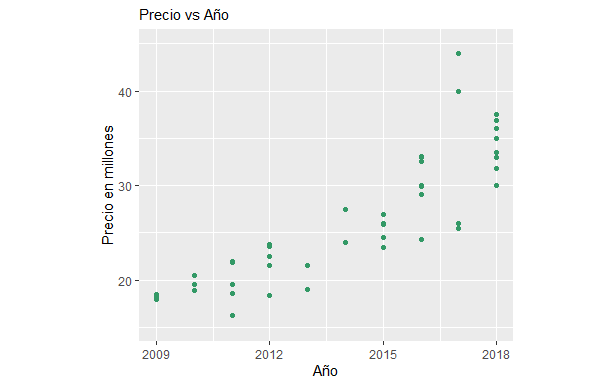
\includegraphics[scale=1]{PvsA}
	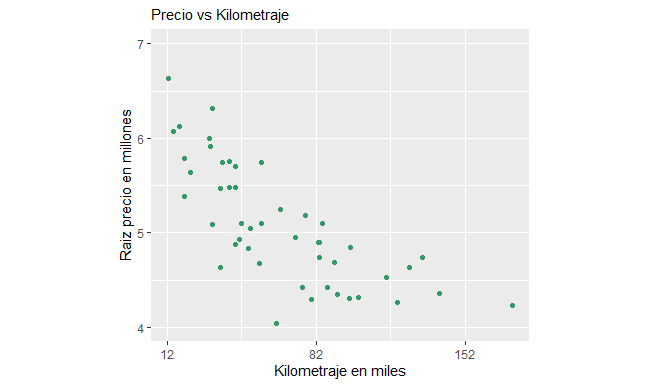
\includegraphics[scale=1]{PvsK}\\
	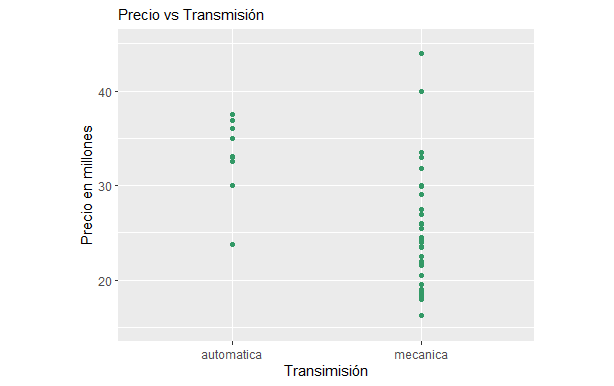
\includegraphics[scale=1]{PvsT}
	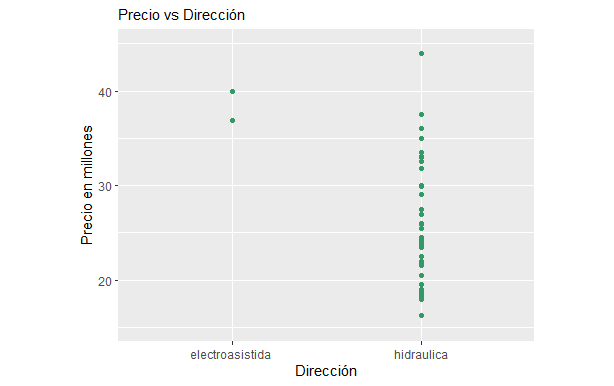
\includegraphics[scale=1]{PvsD}\\
	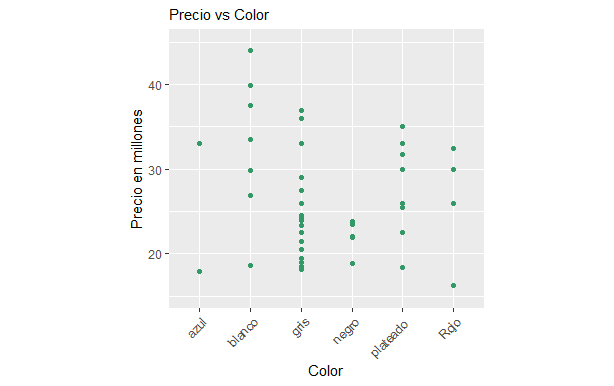
\includegraphics[scale=1]{PvsC}
	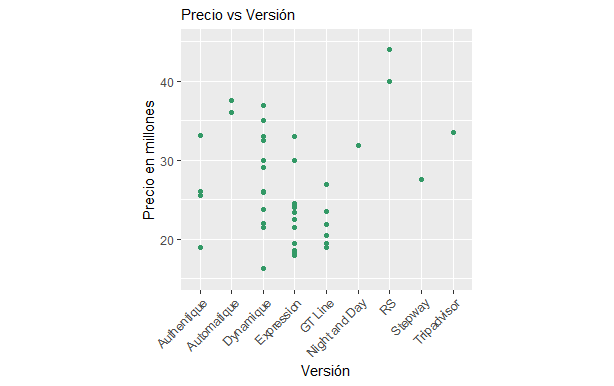
\includegraphics[scale=1]{PvsV}
\end{center}

De acuerdo con \'estas, se ha decidido descartar a $X_6= \text{Direcci\'on}$ como posible variable regresora, dado que tiene s\'olo dos registros diferentes a hidr\'aulica. 

\section*{\textcolor{ginger}{\huge Selecci\'on del modelo}}

Se ha realizado una regresi\'on \textit{stepwise} hacia adelante incluyendo en primera instancia la variable con mayor significancia de manera individual, para el caso estudiado en este trabajo, dicha variable es $X_1=\text{A\~no}$; a este modelo lineal simple se le a\~nadieron las variables $X_3=\text{Versi\'on}$, $X_4=\text{Transmisi\'on}$, $X_5=\text{Color}$, en ese orden; para esto, hicimos uso de los modelos anidados y las tablas anova. Obteniendo as\'i, el modelo de regresi\'on lineal m\'ultiple $$lm(Y \sim X_{1} + X_{3} + X_{4} + X_{5})$$ 

\begin{center}

\begin{tabular}{l c}
	Coefficients  &           \\
	              & Estimate    \\
	(Intercept)   &-312.51104 \\
	a\~no         &   0.15783\\
	versi\'onAutomatique  &   0.29917 \\ 
	versi\'onDynamique    &   0.30790\\ 
	versi\'onExpression   &   0.19132 \\ 
	versi\'onGT Line      &   0.40644  \\ 
	versi\'onNight and Day&   0.36857\\ 
	versi\'onRS           &   1.29756 \\
	versi\'onStepway      &   0.56390  \\ 
	versi\'onTripadvisor  &   0.45271\\
	transmisi\'onMec\'anica     &  -0.43936 \\ 
	colorBlanco       &  -0.20955  \\ 
	colorGris         &  -0.23331  \\ 
	colorNegro        &  -0.23768  \\  
	colorPlateado     &  -0.27418   \\  
	colorRojo         &  -0.44327 \\ 

\end{tabular}
\end{center} 

Al iniciar la regresi\'on stepwise con $X_{1}$ fija, se encuentra que $X_3=\text{Versi\'on}$ es la m\'as significativa para el modelo. Sin embargo, al tener $X_{1}$ y $X_{3}$ fijas, $X_2=\text{Kilometraje}$ no es significativa para \'este y por el contrario, $X_4=\text{Transmisi\'on}$ s\'i lo es. Se procede a analizar la base de datos para encontrar el por qu\'e de este hecho y se encuentran kilometrajes iguales con precios que distan mucho entre s\'i. Finalmente, al modelo $lm(Y\sim  X_{1} + X_{3} + X_{4})$ se le agrega $X_{5}=\text{Color}$ pues como se ve en el siguiente gr\'afico, al menos un color es significativo todos los a\~nos.

\begin{center}
	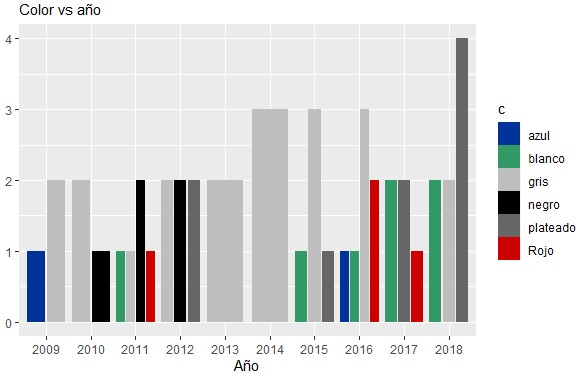
\includegraphics[scale=1.5]{Colorvsa}
\end{center} 

\subsection*{\textcolor{ginger}{Interpretaci\'on}}

\begin{itemize}
	\item Dejando las dem\'as variables constantes, por cada a\~no que aumente el modelo, se aumenta el precio en 0.158 millones de pesos.
	\item Dejando las dem\'as variables constantes, las versiones Automatique, Dynamique, Expression, GT line, Night and Day, RS, Stepway y Tripadvisor son respectivamente 0.30, 0.31, 0.19, 0.41, 0.37, 1.30  y 0.56 millones de pesos m\'as caros que el nivel de referencia  Authentique.
	\item Dejando las dem\'as variables constantes, los colores blanco, gris, negro, plateado y rojo, son  respectivamente 0.21, 0.23, 0.24, 0.27 y  0.44 millones de pesos m\'as baratos que el nivel de referencia azul.
	\item Dejando las dem\'as variables constantes, la transmisi\'on m\'ecanica es 0.44 millones de pesos m\'as barata que la transmisi\'on autom\'atica. 
	
\end{itemize}
\section*{\textcolor{ginger}{\huge Normalidad de los residuos}}

Se realiza el test de normalidad a los residuales del modelo y se concluye que en efecto son normales. Al graficar \'estos contra los valores ajustados por el modelo, se obtiene:
\begin{center}
	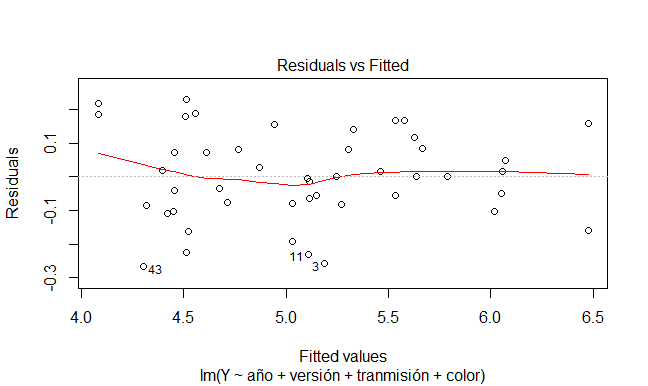
\includegraphics[scale=1.5]{Residuals}
\end{center}


\section*{\textcolor{ginger}{\huge Ejemplo}}
Para un Sandero Dynamique modelo 2015, color blanco y de $60.000$km se tiene el siguiente estimativo:\\
\begin{itemize}
	\item Si la transmisi\'on es autom\'atica:  $Y=-312.51104+(0.15783\times2015)+0.30790-0.20955 = 5.61476 $ as\'i el precio ser\'ia 31.5 millones de pesos.
	\item Si la tranmisi\'on es mec\'anica: $Y=-312.51104+(0.15783\times2015)+0.30790-0.20955-0.43936 = 5.1754 $ as\'i el precio ser\'ia 26.8 millones de pesos.
\end{itemize}


\section*{\textcolor{ginger}{\huge Referencias}}

\begin{enumerate}
	\item V, N\'u\~nez Ant\'on \& F. Tussel. ``Regresi\'on y An\'alisis de Varianza", 2007.
	\item Montgomery, Douglas C. \& Peck, Elizabeth A. \& Vining, G. Geoffrey. ``Introduction to Linear Regression Analysis", Fifth Edition, Wiley.
\end{enumerate}

\end{multicols}
\end{document}